\documentclass[slidetop, mathserif, dvipsnames]{beamer}

% \mode<presentation>
% {
% 	\usetheme{Warsaw}
% 	\setbeamercovered{transparent}
% }

% \usepackage{caption}
\usepackage{subcaption}
\captionsetup{compatibility=false}

% \usepackage[dvipsnames]{xcolor}

\mode<presentation>{
	\usetheme{Berlin}
	\setbeamercovered{transparent}
	\usefonttheme{professionalfonts}
}

\usepackage{amsmath, amsfonts, amssymb}
\usepackage{mathrsfs,dsfont}

\newcommand{\norm}[1]{\left\|#1\right\|}
\newcommand{\suchthat}{-\hspace{-10pt}\ni\hspace{-10pt}-}


\AtBeginSection[]
{
   \begin{frame}
       \tableofcontents[currentsection]
   \end{frame}
}

\addtobeamertemplate{navigation symbols}{}{%
    \usebeamerfont{footline}%
    \usebeamercolor[fg]{footline}%
    \hspace{1em}%
    \insertframenumber/\inserttotalframenumber
}

%% want to use verbatim: \begin{frame}[fragile]

\title[Metrics for Tracking]{Metrics for Evaluating Trackers}
\author[chy1010]{Chien, Hung-Yu \\ {\small\tt hungyu@linkernetworks.com}}
\date{\today}

\begin{document}

\begin{frame}
	\titlepage
\end{frame}

\section[Outline]{}
\begin{frame}
	\frametitle{Outlines}
	\tableofcontents
\end{frame}



\section{Trackers and Multiple Object Tracking}

\begin{frame}
	\frametitle{What is a tracker?}

	A {\bf tracker} is a \emph{model} or a \emph{post-processor}
	that performs on a video, i.e. a sequence of image frames.

	\quad

	A tracker model is often used on MOT (multiple object tracking) tasks,
	which consists of
	\begin{itemize}
	\item
		to detect objects inside each frames, and
	\item
		to recognize if the detections in consecutive frames are the
		same or not.
	\end{itemize}

	\quad

	We also use the term `tracker' to indicate the recognization part
	in particular. In this case, trackers are often seem as post-processors
	in model pipelines.

\end{frame}



\begin{frame}
	\frametitle{Inference Results of a Tracker}

	Unlike SOT (single object tracking), MOT are mainly to deal with
	multiple objects of \underline{one category}.
	And a tracker should assign
	an identity to each detected object along a video file or a video
	stream.

	\begin{figure}
		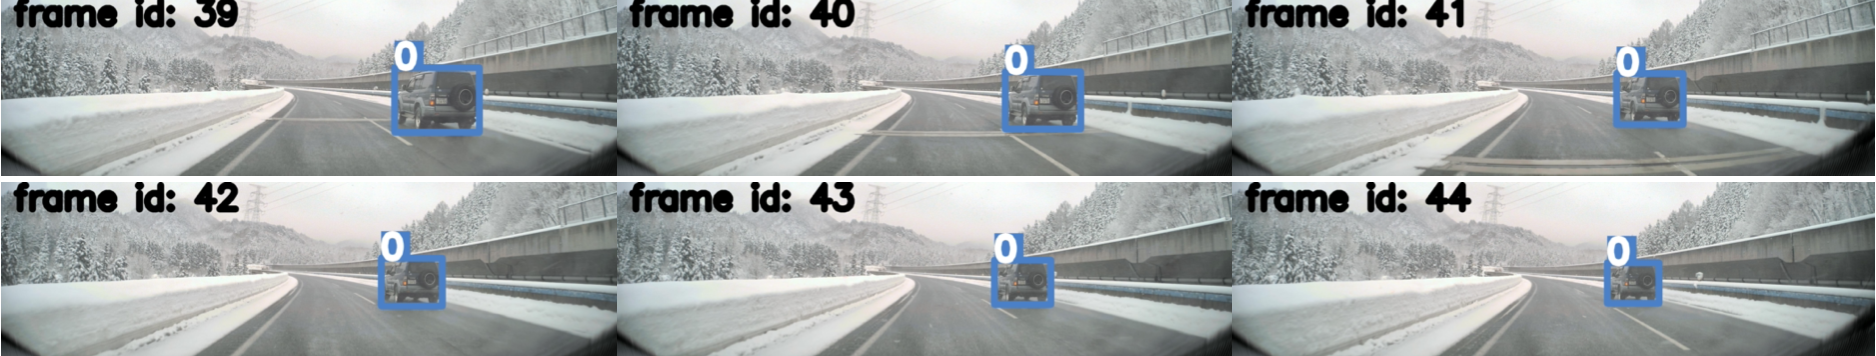
\includegraphics[width=1.05\textwidth]{pics/track01.png}
		\caption{Detect \& track objects on continuous frames.}
	\end{figure}

\end{frame}

\begin{frame}
	\frametitle{Inference Results of a Tracker}

	Finally, the inference results should \emph{locate objects},
	\emph{maintain their ids},
	and \emph{yield individual trajectories}.

	\begin{figure}
		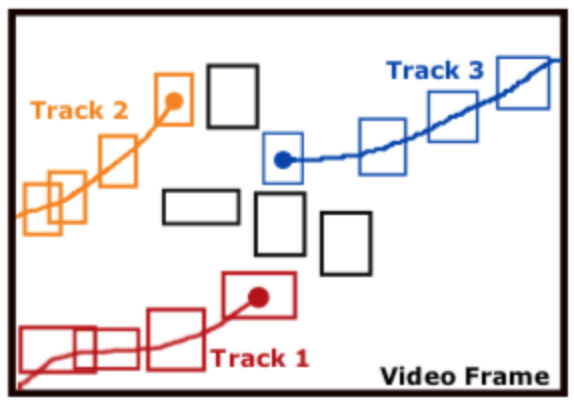
\includegraphics[height=90pt]{pics/fig1.png}
		\caption{Trajectories and several un-tracked / isolated detections.}
	\end{figure}

\end{frame}

\begin{frame}
	\frametitle{To Evaluate a Tracker}

	To evaluate a tracker, we compare the inference results with ground-truths.

	\quad

	Similarly, the ground-truths also contain
	\begin{itemize}
	\item \emph{locations of objects} (denoted by gtObjs, gtDets) and
	\item their \emph{identities}.
	\end{itemize}
	And objects with the same id also form a trajectory.

	\quad

	A {\bf metric} here is used to measure the difference between
	ground-truths and the predictions (hypotheses).

\end{frame}

\begin{frame}
	\frametitle{To Evaluate a Tracker}

	We think a tracker is {\bf good} if
	\emph{the ids it assigns to the same objects are consistent in different frames}.
	However, this is also based on the performance of its detection part.

	\begin{figure}
		\begin{subfigure}{.48\textwidth}
		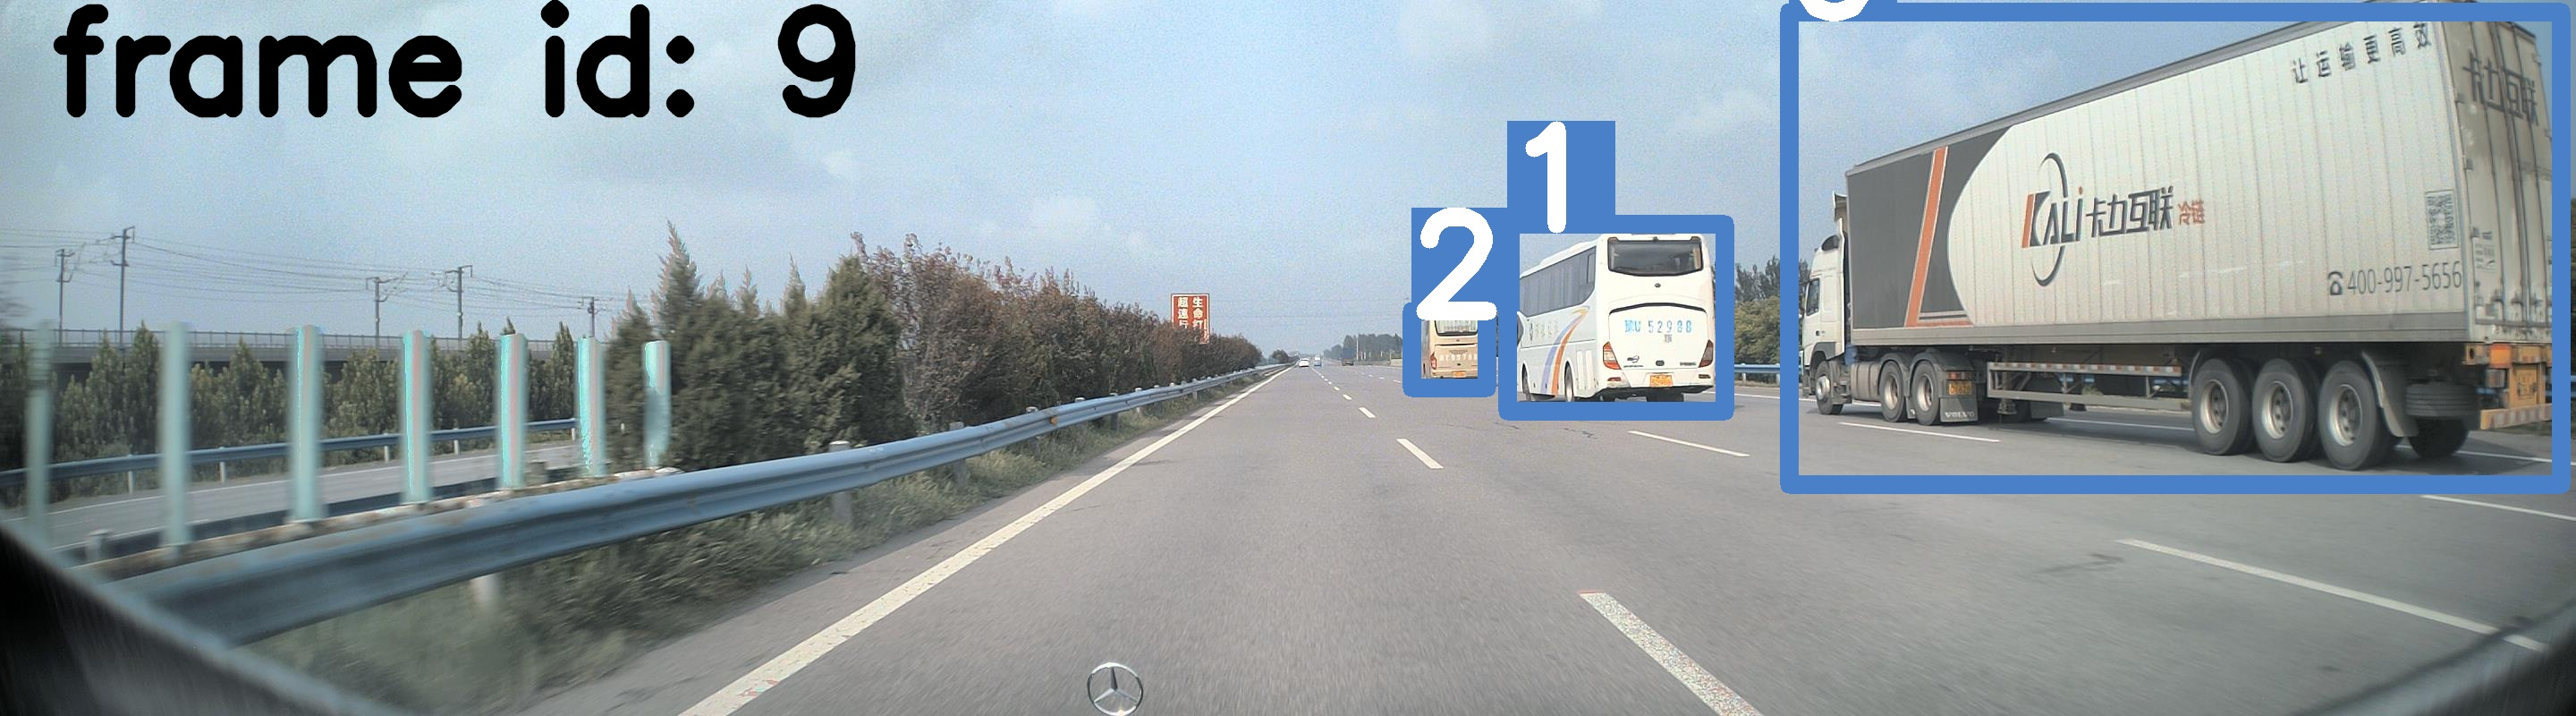
\includegraphics[width=150pt]{pics/track03.jpg}
		\end{subfigure}
		\begin{subfigure}{.48\textwidth}
		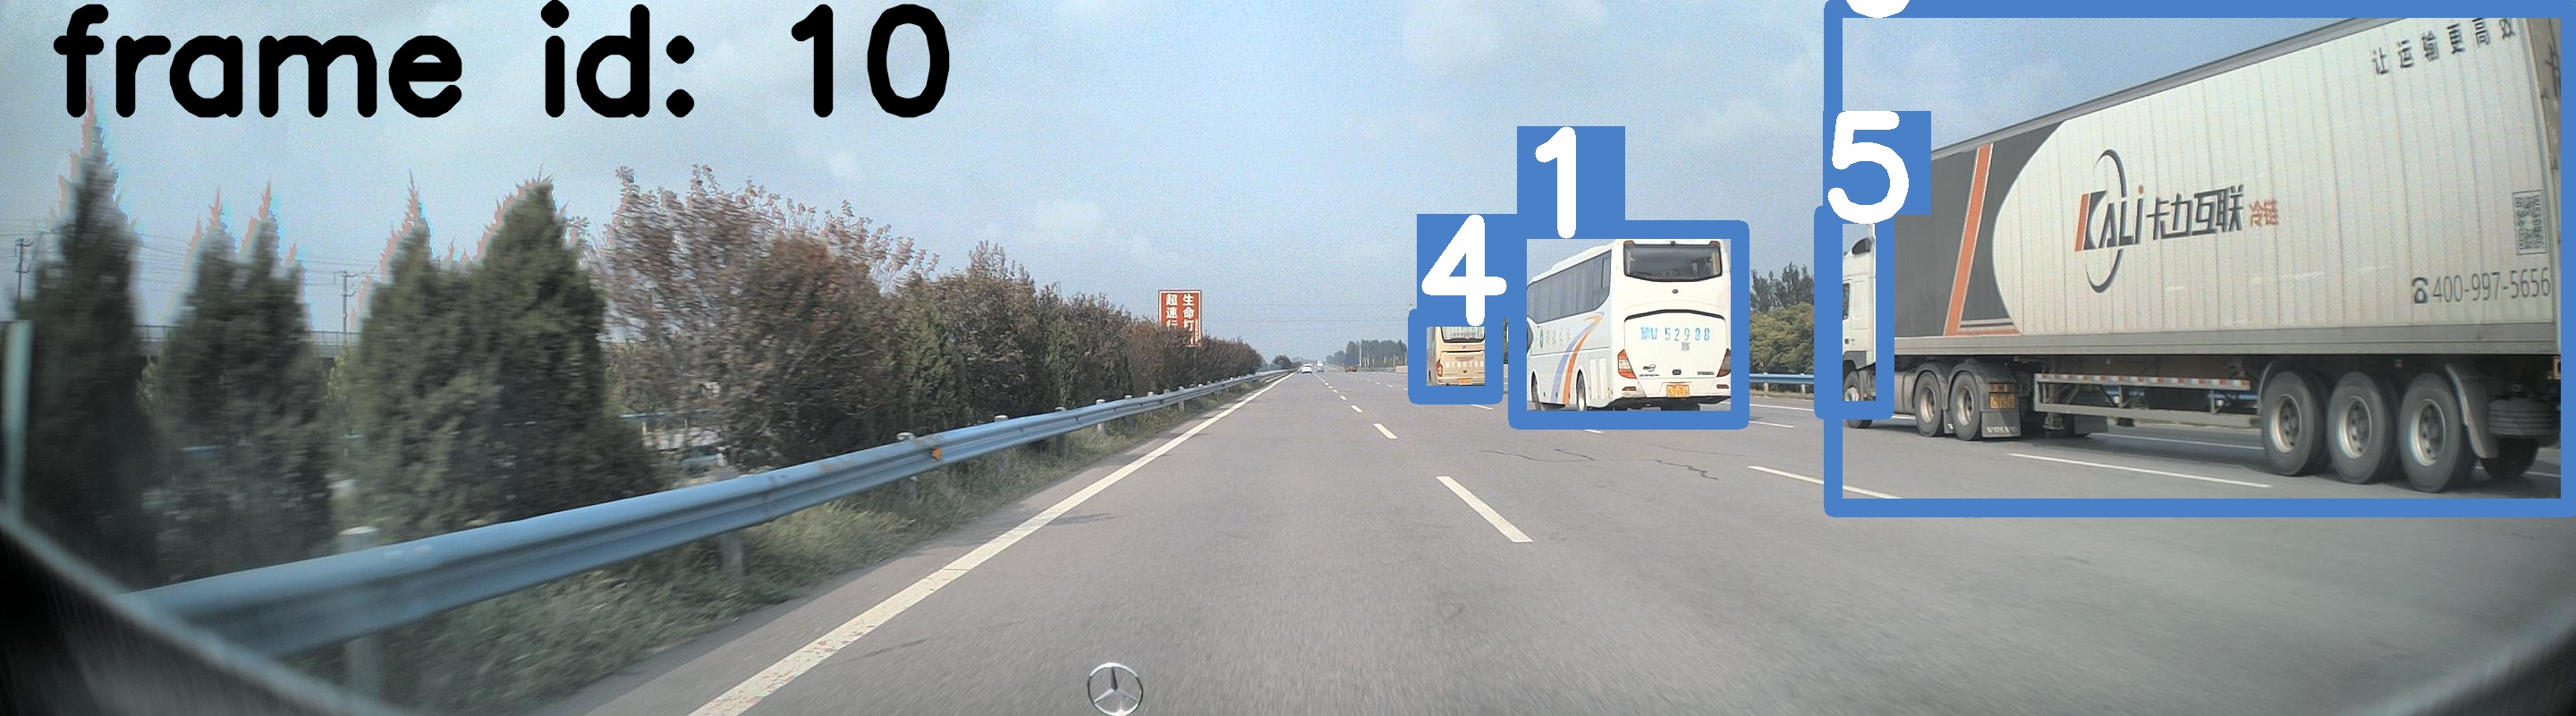
\includegraphics[width=150pt]{pics/track04.jpg}
		\end{subfigure}
		\caption{{\color{red}\bf [NG cases]} Fail to track the id 2.
			Wrong detection on the id 5.}
	\end{figure}

	To do this, we firstly match detections to the ground-truths
	and see further if objects and ids are correctly tracked.

\end{frame}

\section{Matchings and Associations}

\begin{frame}
	\frametitle{Matching in Detection Levels}
			
	The matchings are done according to their {\bf similarity scores}.
	
	$\max\{1-\text{dist}, 0\}$ or IoU
	are often used as scoring functions.
			
	\begin{figure}
		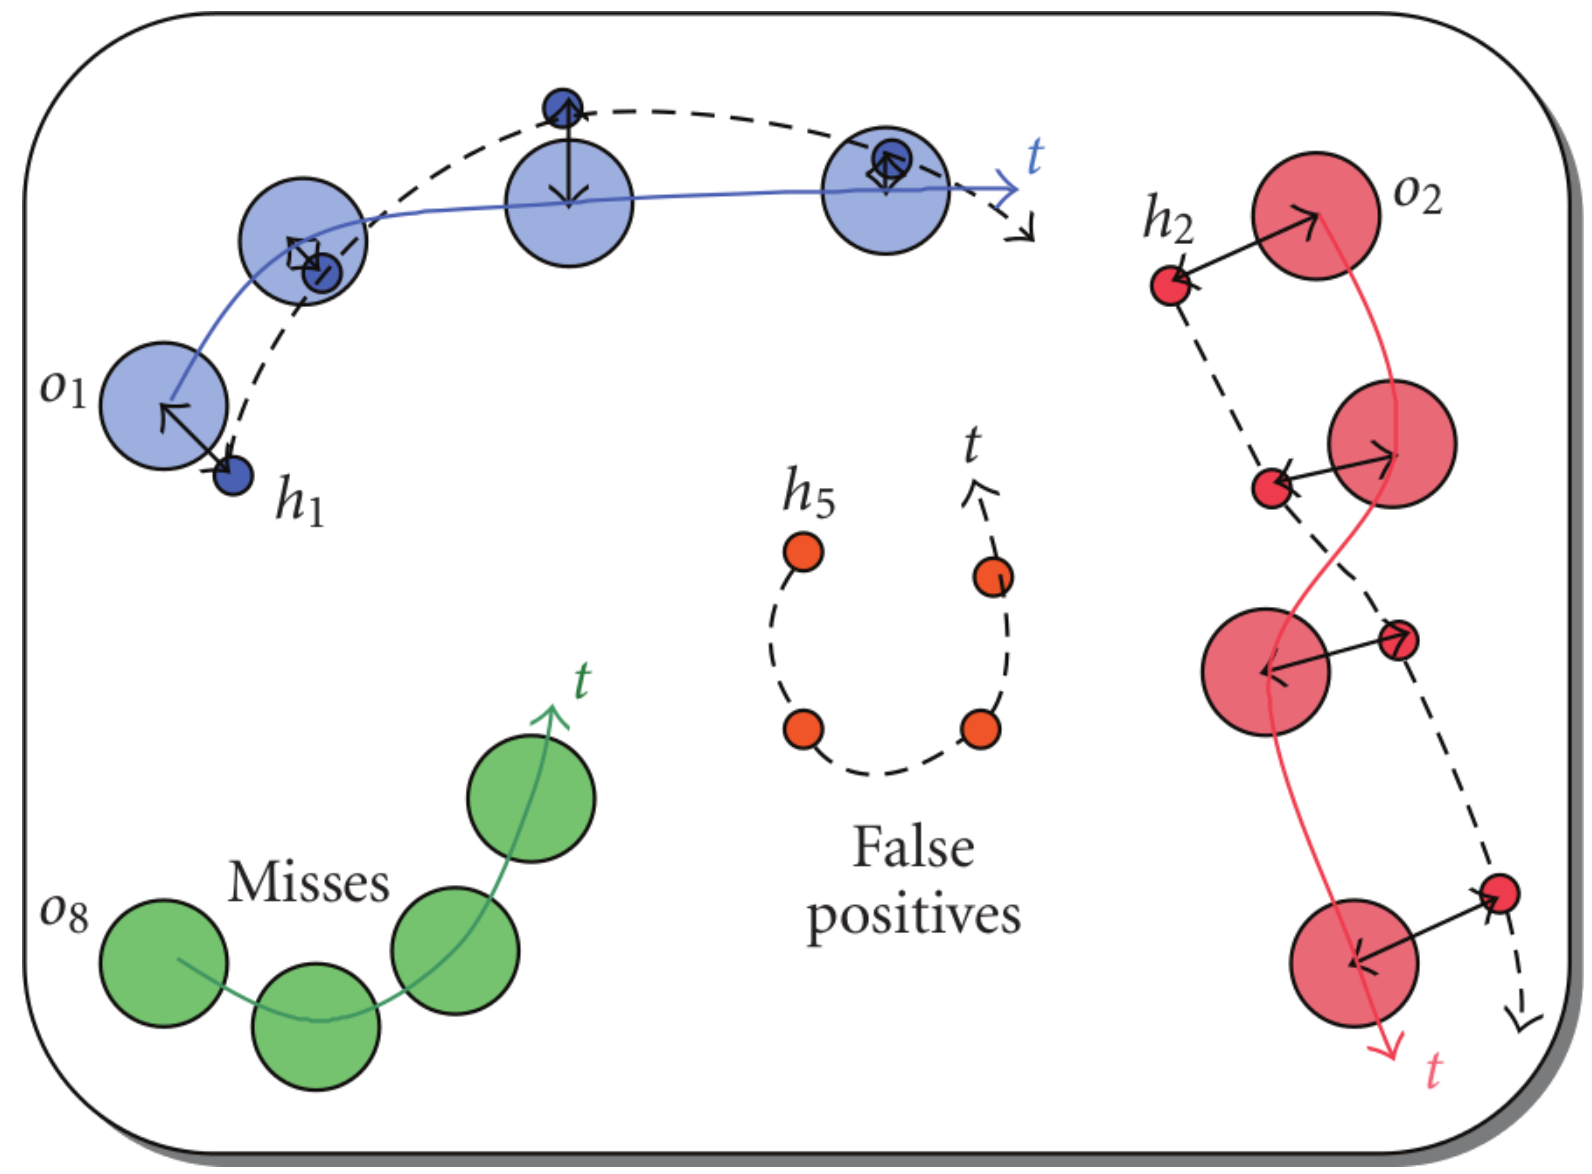
\includegraphics[width=150pt]{pics/fig2.png}
		\caption{Matchings (1-1 relation), false positives and misses in consecutive frames.
		Here the similarity is measured by the central distances.}
	\end{figure}

\end{frame}

\begin{frame}
	\frametitle{Similarity Threshold and the Performance Measures}
		
	Denote the similarity function by $\mathcal S$.
	To filter out bad matches, a threshold $\alpha$ is given.
	Once a matching $\Pi_\alpha$ under threshold $\alpha$ is done, it satisfies
	\[
		\forall\ (g,p)\in\Pi_\alpha, ~ \mathcal S(g,p) \geq \alpha.
	\]
	Hence we can define the following measures in the detection level.
	\begin{itemize}
		\item TP, TP$_\alpha$: matched pairs in a matching $\Pi_\alpha$.
		\item FP, FP$_\alpha$: non-matched predictions.
		\item FN, FN$_\alpha$: non-matched ground-truths.
	\end{itemize}
	{\color{red} Remark: For an $\alpha$, there may be several matchings fulfilling this threshold.}
\end{frame}

\begin{frame}
	\frametitle{Notations}
			
	\begin{itemize}
		\item A matching $\Pi$ can be a matching in a frame $f$ and specified by $\Pi^{(f)}$;
		      or be a matching during all frames.
		\item When $\Pi$ denotes a global matching of objects, it is the union of all its sections:
		      $\Pi = \cup_{f\in F}\Pi^{(f)}$ ($F$ collection of all frames).
		\item Furthermore, once a set $E$ is well-defined in each frame,
		      we denote $E^{(f)}$ as the $f$-section, i.e. elements in frame $f$.
		      		      		      
	\end{itemize}
			
	\vspace{-2pt}

	For a ground-truths $g$ or a prediction $p$, denote
	\begin{itemize}
		\item $f_g$ / $f_p$ as the frame it appears;
		\item $\text{gtId}(g)$ / $\text{prId}(p)$ as its id;
		\item $\text{gtTr}(g)$ / $\text{prTr}(p)$ as its trajectory.
	\end{itemize}

\end{frame}

\begin{frame}
	\frametitle{IDSW in Consecutive Frames}
			
	An {\bf IDSW (id switch)} event means there exist TP pairs, say $(g_i, p_j)\in\Pi^{(f)}$,
	$(g_k, p_\ell)\in\Pi^{(f+1)}$, in two consecutive frames
	$f$ and $f+1$ that satisfy
	\[
		\text{gtId}(g_i) = \text{gtId}(g_k),\ 
		\text{prId}(p_j) \neq \text{gtId}(p_\ell).
	\]
	Actually, this is an \emph{id mismatch} occuring in frame $f+1$.
	If two detections exchange their ids in a new frame,
	then this is regarded as two IDSW events.
	\begin{figure}
		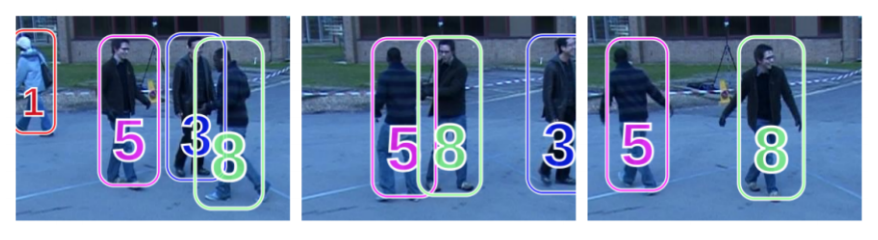
\includegraphics[width=180pt]{pics/fig3.png}
		\caption{The ids 3 \& 8 exchanges. Two IDSW events.}
	\end{figure}
			    
\end{frame}

\begin{frame}
	\frametitle{IDSWs Caused by ID-Exchange and Losing Tracks}

	\begin{figure}
		\begin{subfigure}{.49\textwidth}
			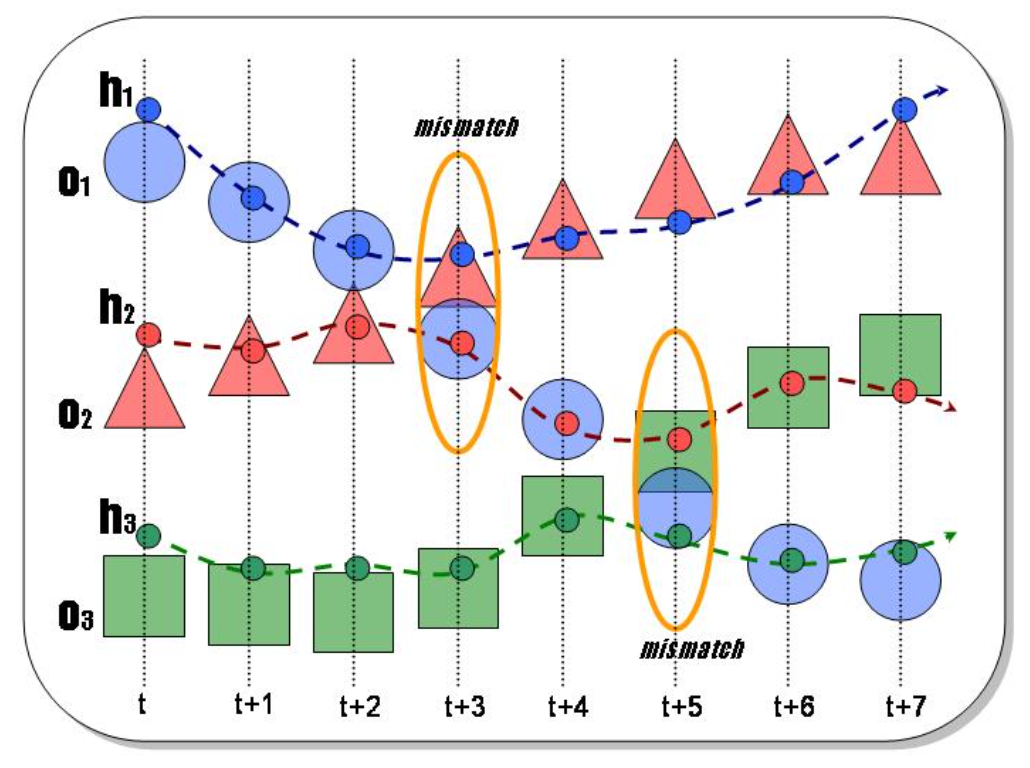
\includegraphics[width=150pt]{pics/fig16.png}
		\end{subfigure}
		\begin{subfigure}{.49\textwidth}
			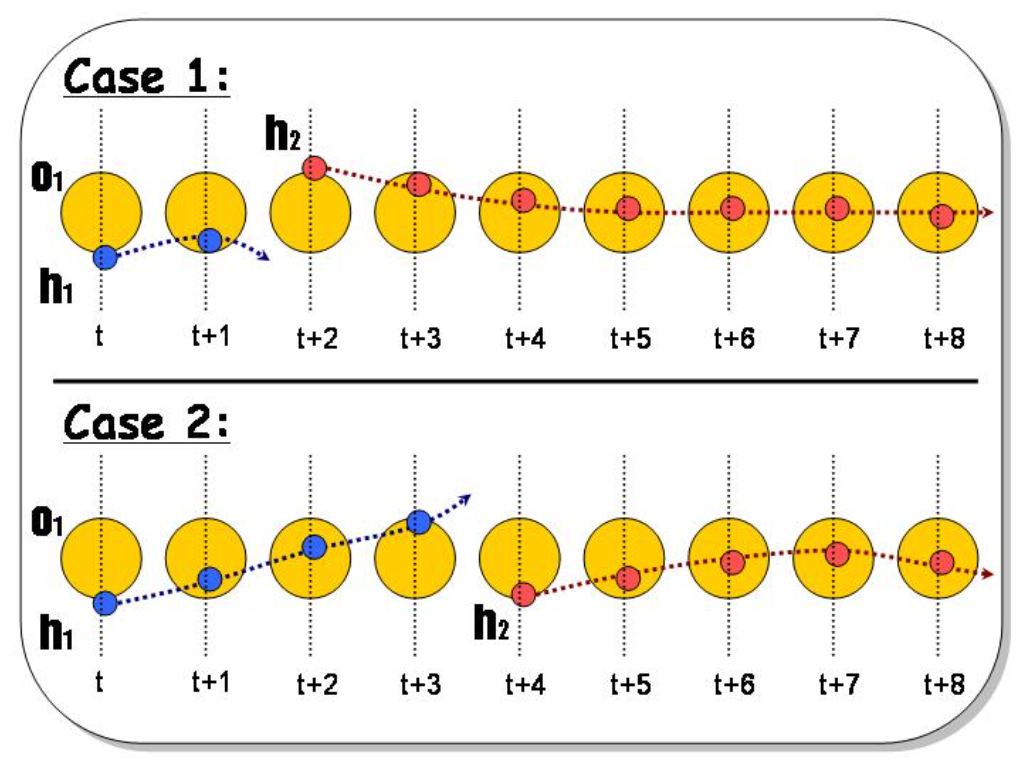
\includegraphics[width=150pt]{pics/fig17.png}
		\end{subfigure}
		\caption{Cases of losing tracks.}
	\end{figure}
\end{frame}

\begin{frame}
	\frametitle{Tracking Accuracy: A First Meet.}

	Now %by utilizing measures introduced above,
	we have a simple metric to evaluate the performance.
	Instead of measuring the difference,
	we'd like to use a `score` to present how good it is.

	\vspace{3pt}

	The tracking errors consist of:
	\begin{itemize}
	\item \emph{an id switch event}, or that
	\item \emph{an object is out of detection}, or a \emph{wrong prediction}.
	\end{itemize}

	The MOTA (multiple object tracking accuracy) score is defined by
	\[
		\text{MOTA} = 1 - \dfrac{|\text{FP}| + |\text{FN}| + |\text{IDSW}|}{|\text{gtDets}|}.
	\]
	The range of MOTA is $(-\infty,1]$. As FP, FN, IDSW increase, the MOTA value decrease.

\end{frame}

\begin{frame}
	\frametitle{Example: MOTA score}

	\begin{figure}
		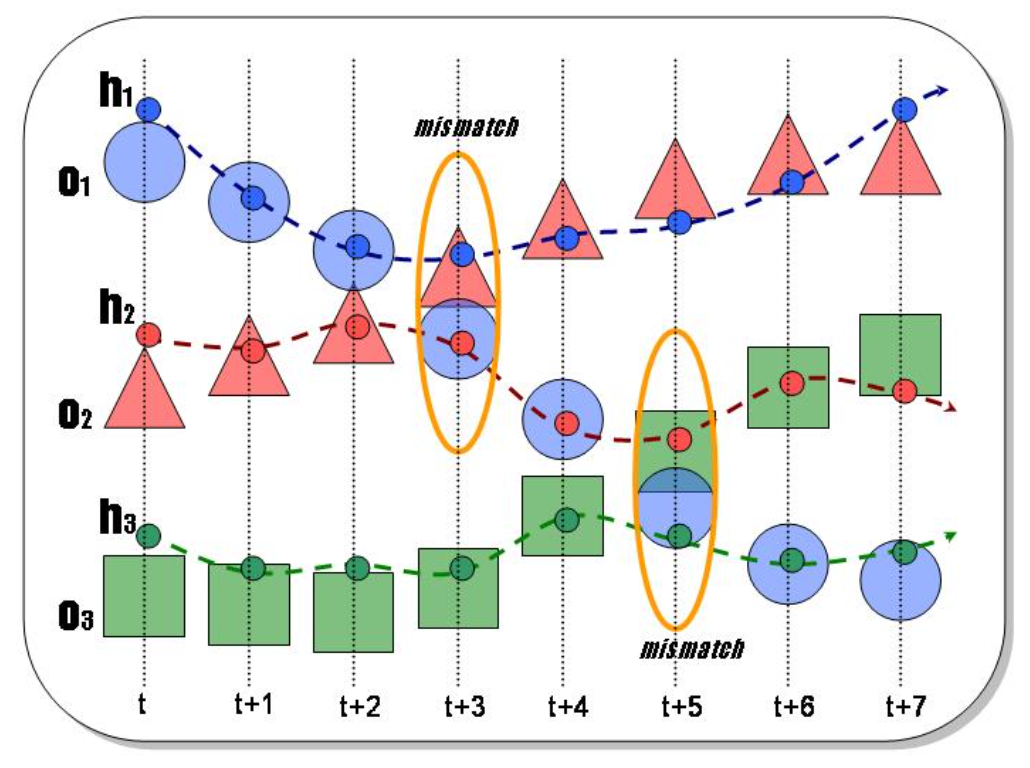
\includegraphics[width=200pt]{pics/fig16.png}
		\caption{24 TP, 0 FP, 0 FN, 4 IDSW: MOTA $=1-4/24 = 5/6 \approx 83\%$.}
	\end{figure}
\end{frame}


\begin{frame}
	\frametitle{Discussion on MOTA}

	\begin{minipage}{50pt}
		\begin{figure}
			
\includegraphics[width=50pt]{pics/question2.png}
		\end{figure}
	\end{minipage}
	\begin{minipage}{250pt}
	\begin{itemize}
	% \item Which hypothesis id is matched to ground-truth id? for most frames?
	\item When MOTA is much lower from $1$, we don't know either detectors or tracking result is worse.
	\item Sometimes IDSW can't help distinguish the exchange of two ids or
		losing and re-tracking an object with id.
	\end{itemize}
	\end{minipage}

	\vspace{10pt}

	In the following, matching in a trajectory level is investigated.

\end{frame}

% \subsection{Matching in Trajectory Levels}

\begin{frame}
	\frametitle{Matching in Trajectory Levels}

	A sketch of a matched pair of trajectories.
	\begin{figure}
		\begin{subfigure}{.5\textwidth}
			\centering
			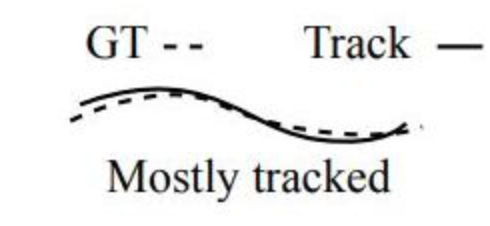
\includegraphics[width=130pt]{pics/fig4.png}
		\end{subfigure}%
		\begin{subfigure}{.5\textwidth}
			\centering
			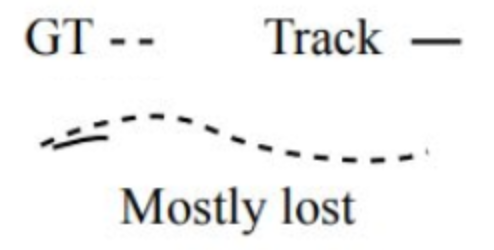
\includegraphics[width=115pt]{pics/fig5.png}
		\end{subfigure}
		\caption{Mostly tracked \& mostly lost.}
	\end{figure}

	\vspace{-5pt}

	A trajectory-to-trajectory matching $\leftrightarrow$ A gtid-to-prid matching.
	
	\quad

	To match trajectories, the similarity scores of trajectories are
	measured by the similarities of detections.
			
\end{frame}

\begin{frame}
	\frametitle{Similarity of Trajectories}
			
	For each pair of trajectories,
	we can count the number of objects of the overlapping and the rest parts.
			
	\vspace{5pt}
			
	Let $\mathfrak g$, $\mathfrak p$ be a pair
	and $\alpha$ be a (detection-) similarity threhold.
	We can also define the analogues:

	\vspace{5pt}

	\begin{itemize}
		\item $\mathds{TP}$, $\mathds{TP}_{\mathfrak g, \mathfrak p}$:
		      the overlapping part of $\mathfrak g$ and $\mathfrak p$.
		      \[
		      	\mathds{TP} := \{(g,p)\ |\ 
		      	g\in\mathfrak g,~
		      	p\in\mathfrak p,~
		      	f_g=f_p,~ \mathcal S(g,p)\geq \alpha\}
		      \]
		\item $\mathds{FP}$, $\mathds{FP}_{\mathfrak g, \mathfrak p}$:
		      the non-matched predictions.
		      \begin{align*}
		      	\mathds{FP} := & \{ p\in\mathfrak p\ |\ 
		      	\nexists\ g\in\mathfrak g ~\suchthat~ \mathcal S(g,p)\geq\alpha,~ f_g=f_p.\}
		      \end{align*}
	\end{itemize}
			
\end{frame}

\begin{frame}
	\frametitle{Similarity of Trajectories}
			
	\begin{itemize}
		\item $\mathds{FN}$, $\mathds{FN}_{\mathfrak g, \mathfrak p}$: the non-matched ground-truth objects.
		      \begin{align*}
		      	\mathds{FN} := & \{ g\in\mathfrak g\ |\ 
		      	\nexists\ p\in\mathfrak p ~\suchthat~ \mathcal S(g,p)\geq\alpha,~ f_p=f_g.\}
		      \end{align*}
	\end{itemize}
			
	The similarity of trajectories is defined by
	\[
		\mathcal S_{\rm tr}(\mathfrak g, \mathfrak p) :=
		\dfrac{|\mathds{TP}_{\mathfrak g,\mathfrak p}|}{
			|\mathds{TP}_{\mathfrak g,\mathfrak p}|+|\mathds{FP}_{\mathfrak g,\mathfrak p}|+|\mathds{FN}_{\mathfrak g,\mathfrak p}|
		}
	\]
	Once the similarities are calculated,
	the matching of trajectories can be done by a Hungarian algorithms.
\end{frame}


\begin{frame}
	\frametitle{Performance Measures Focusing on IDs}
			
	Suppose a matching of trajectories are done and denoted by $\mathfrak P$,
	we can define the performance measures as follows.
			
	\vspace{4pt}
			
	Again, denote $\alpha$ as the (detection-) similarity threshold.
	\begin{itemize}
		\item IDTP:
		      the overlapping part of all $(\mathfrak g, \mathfrak p) \in \mathfrak P$.
	\end{itemize}
			
	\vspace{-15pt}
	\[
		\text{IDTP} := \left\{ (g,p)\ |\ 
		g\in\mathfrak g, ~ p\in\mathfrak p, ~
		f_g=f_p, ~ 
		\mathcal S(g,p) \geq \alpha, ~ 
		(\mathfrak g, \mathfrak p)\in\mathfrak P
		\right\}
	\]
	\vspace{-10pt}
	\begin{itemize}
		\item IDFP:
		      non-matched predictions in matched pairs
		      and all predictions in non-matched predictive trajectories.
	\end{itemize}
	\begin{align*}
	\text{IDFP} := & \left\{ p\in\text{prDets}\ \left|\                                                
	\mathcal S(g,p)<\alpha, \ 
	\forall\ g\in\mathfrak g^{(f_p)},
	(\mathfrak g,\mathfrak p)\in\mathfrak P.
	\right.
	\right\} \\
					& \bigcup \left\{p \in \text{prDets}\ |\ \text{prTraj$(p)$ is not matched.}\right\} 
	\end{align*}
			    
\end{frame}

\begin{frame}
	\frametitle{Performance Measures Focusing on IDs}
	\begin{itemize}
		\item IDFN:
		      non-matched ground-truths in matched pairs and
		      all ground-truths in non-matched ground-truth trajectories.
	\end{itemize}

	\vspace{-15pt}
	\begin{align*}
		\text{IDFN} := & \left\{ g\in\text{gtDets}\ \left|\                                                
		\mathcal S(g,p)<\alpha, \ 
		\forall\ p\in\mathfrak p^{(f_g)},
		(\mathfrak g,\mathfrak p)\in\mathfrak P
		\right.
		\right\} \\
		               & \bigcup \left\{g \in \text{gtDets}\ |\ \text{gtTraj$(g)$ is not matched}\right\}. 
	\end{align*}
	
	By these quantities, the id-matchings can be evaluated by
	\[
		\text{ID-Precision} := \dfrac{|\text{IDTP}|}{|\text{IDTP}| + |\text{IDFP}|},
		\quad
		\text{ID-Recall} := \dfrac{|\text{IDTP}|}{|\text{IDTP}| + |\text{IDFN}|},
	\]

	\vspace{-10pt}
	\[
		\text{IDF1} := \dfrac{|\text{IDTP}|}{|\text{IDTP}| + 0.5|\text{IDFP}| + 0.5|\text{IDFN}|}.
	\]
\end{frame}

\begin{frame}
	\frametitle{Discussion on the ID-Metrics}
			
	By observations, the id-metrics show how good the trackings are.

	\quad
	
	\begin{figure}
		\begin{subfigure}{.5\textwidth}
			\centering
			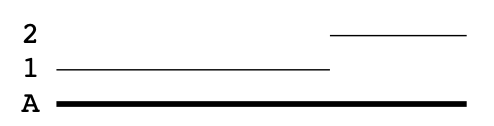
\includegraphics[width=120pt]{pics/fig6.png}
		\end{subfigure}%
		\begin{subfigure}{.5\textwidth}
			\centering
			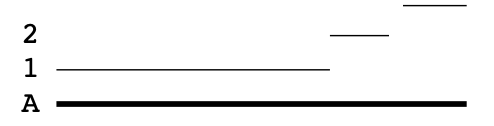
\includegraphics[width=120pt]{pics/fig7.png}
		\end{subfigure}
		% \caption{The id metrics only measure tracking results of matched peices.
		% The ground-truth id is shown by the bold line.}
	\end{figure}
	\begin{minipage}{160pt}
	\begin{align*}
		\text{IDTP} & = \{(g,p)\ |\ g\in A, p\in 1\}, \\
		\text{IDFP} & = \{p\ |\ p\notin 1\}, \\
		\text{IDFN} & = \{g\ |\ g\in A, ~ \nexists\ p\in 1\},
	\end{align*}
	\end{minipage}
	\begin{minipage}{120pt}
		ID-Precision $=$ ID-Recall $=$ ID-F1 $\approx$ $0.75$.
	\end{minipage}

	\vspace{5pt}

	But once if several fragmentations occur in different frames,
	then we cannot not distinguish this case with the mostly lost cases.

\end{frame}

\begin{frame}
	\frametitle{Problems in Matching Trajectories}
			
	\begin{itemize}
		\item {\bf fragmentations}:
		      A ground-turth trajectory is matched by
		      several predictive trajectories.
		\item {\bf merge}:
		      A hypothetical trajectory is matched to several ground-truths.
	\end{itemize}
	
	\vspace{-15pt}
	\begin{figure}
		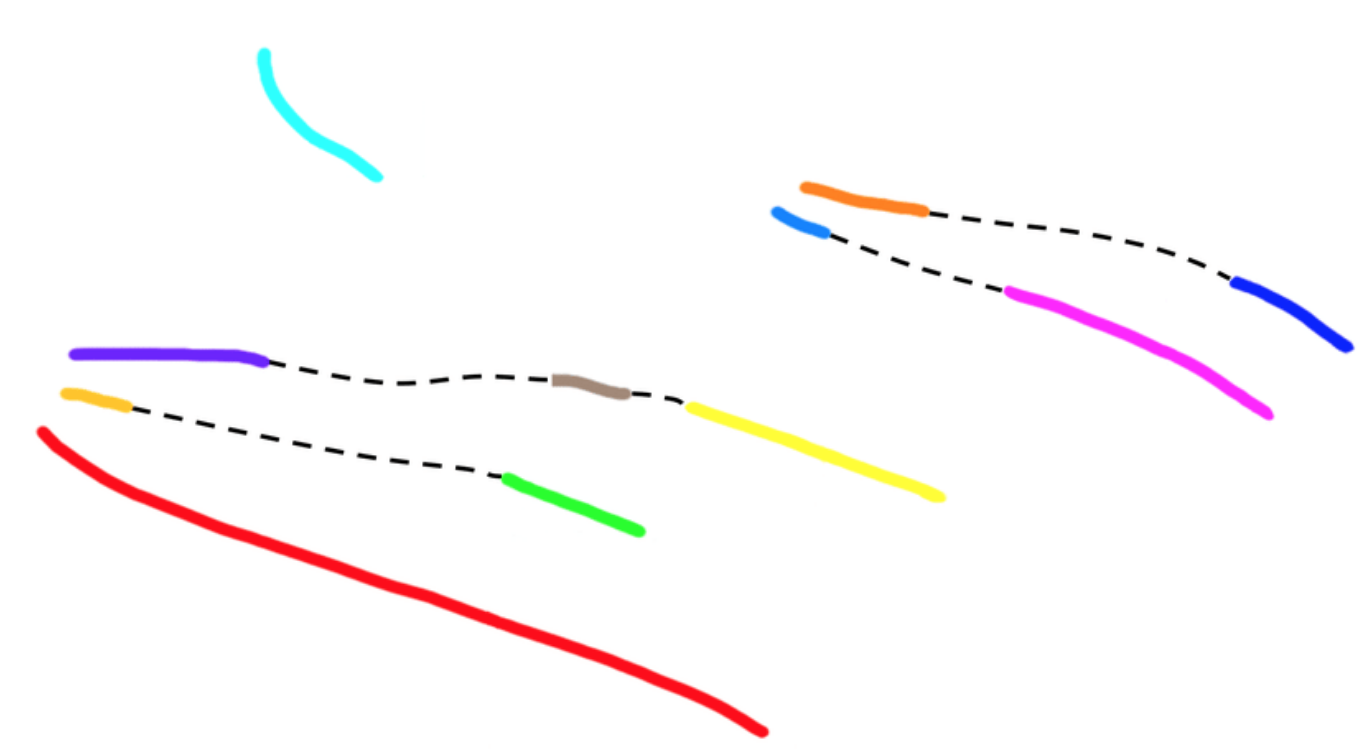
\includegraphics[width=140pt]{pics/fig9.png}
		\caption{Six objects. Colored segm's are diff. ids and dash lines are misses.}
	\end{figure}
		
	% \vspace{-15pt}
	% It's a drawback that trajectory matching only allows 1-1 relation.
			
\end{frame}

\begin{frame}
	\frametitle{Measures for Associations of Objects}
			
	By concepts in id-metrics,
	{\bf tracking associations of a single object} is developed in further.
	\emph{Do matching in a detection level and associate multiple ids during all
	frames by matching.}
			
	\vspace{5pt}
			
	Given a framewise matching $\Pi_\alpha$.
	Let $c = (g,p)$ be a TP pair in a frame.
	We define TPA (true positive associations), FPA (false positive associations)
	and FNA (false negative associations) as follows.
	\begin{align*}
		\text{TPA}(c) :=                       
		\left\{(g_i, p_j)\in\text{TP}\ \left|\ 
		\begin{array}{c}                       
		\text{grId}(g_i)=\text{grId}(g), \\
		\text{prId}(p_j) = \text{prId}(p)      
		\end{array}\right.                     
		\right\}.                              
	\end{align*}
	Note that $|\text{TPA}(c)|$ is also the number of frames that $\text{gtTraj}(g)$
	and $\text{prTraj}(p)$ overlap.
			
\end{frame}

\begin{frame}
	\frametitle{Measures for Associations of Objects}
			
	% Similarly, for the TP pair $c = (g, p)$, we also define the false positive associations
	% and false negative associations as follows.
	\vspace{-20pt}
	\begin{align*}
		\text{FPA}(c) := &             
		\left\{(g_i, p_j)\in\text{TP}\ \left|\ 
		\begin{array}{c}
		\text{grId}(g_i) \neq \text{grId}(g), \\
		\text{prId}(p_j) = \text{prId}(p)
		\end{array}\right.
		\right\} \\
		                 & ~ \bigcup ~ 
		\Big\{p_j\in\text{FP}\ |\ 
		\text{prId}(p_j) = \text{prId}(p)
		\Big\}; \\
		\text{FNA}(c) := &             
		\left\{(g_i, p_j)\in\text{TP}\ \left|\ 
		\begin{array}{c}
		\text{grId}(g_i) = \text{grId}(g), \\
		\text{prId}(p_j) \neq \text{prId}(p)
		\end{array}\right.
		\right\} \\
		                 & ~ \bigcup ~ 
		\Big\{g_i\in\text{FN}\ |\ 
		\text{gtId}(g_i) = \text{gtId}(g)
		\Big\}.
	\end{align*}
	Note that $\text{FPA}(c)$ and $\text{FNA}(c)$ relate to the non-matched
	or id-mismatched objects in $\text{prTraj}(p)$ and $\text{grTraj}(g)$.
			
\end{frame}

\begin{frame}
	\frametitle{Tracking Accuracy of a Single Matched Pair}

	Under a framewise matching, for a TP pair $c=(g,p)$,
	the accuracy of the association of the id-matching $(\text{grId}(g), \text{prId}(p))$
	is
	\[
		\mathcal A(c) := 
		\dfrac{|\text{TPA}(c)|}{|\text{TPA}(c)|+|\text{FPA}(c)|+|\text{FNA}(c)|}.
	\]
	This value shows
	\emph{how good the association $(\text{grId}(g), \text{prId}(p))$ is}.
	And we can compare these accuracies calculated from different pairs
	of id-matchings.

	\vspace{5pt}

	Comparing to the id-metrics, such accuracy $\mathcal A$ gives
	\emph{partial credits} on small peices of associated trajectories.

\end{frame}

\begin{frame}
	\frametitle{An Example of Tracking Associations}
	\begin{figure}
		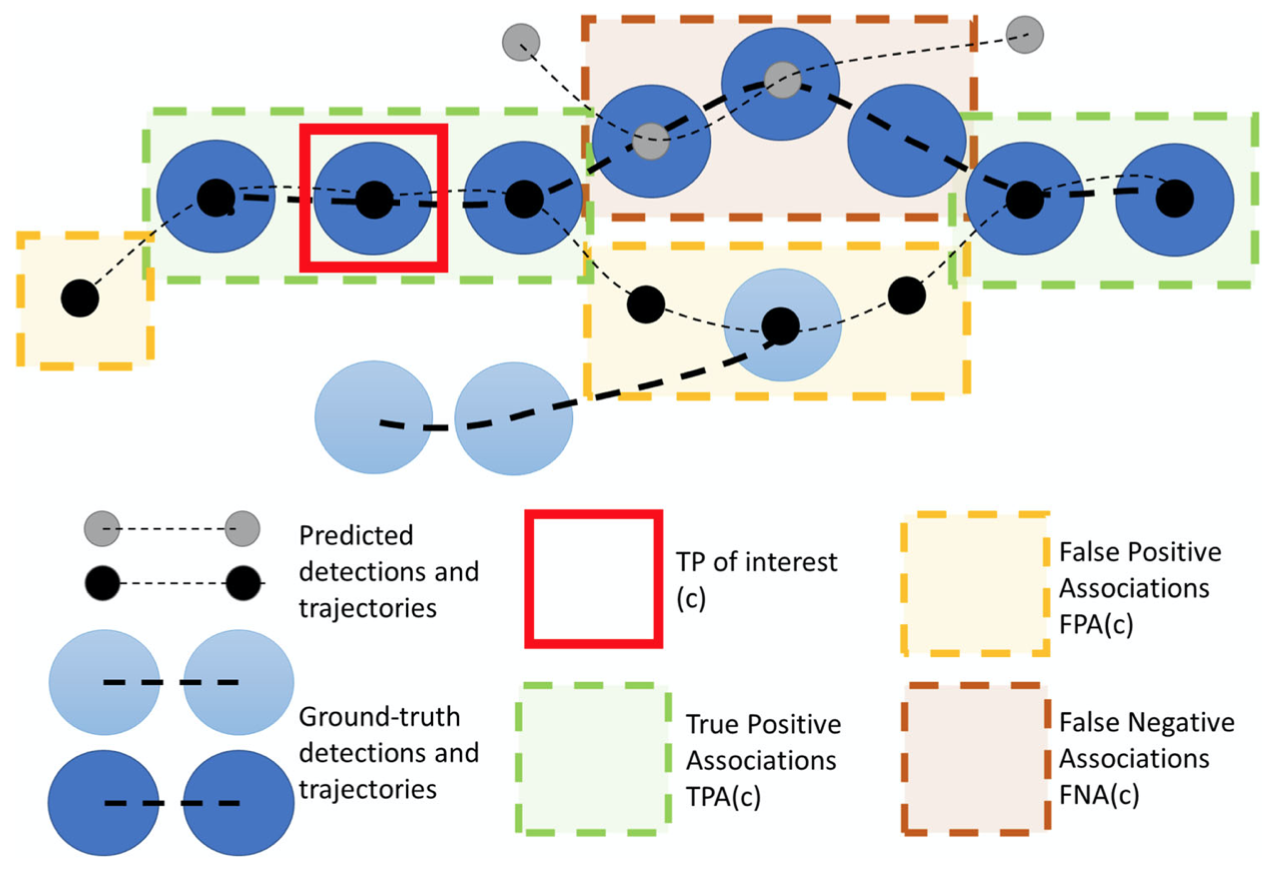
\includegraphics[width=240pt]{pics/fig8.png}
		\caption{For the interested object (red box), TPA: 5; FPA: 4; FNA: 3.}
	\end{figure}
\end{frame}

\begin{frame}
	\frametitle{HOTA Scores: First Look}

	The average AssA (accuracy of associations) is of this form:
	\[
		\text{AssA} = \dfrac{1}{|\text{TP}|} \sum_{c\in\text{TP}} \dfrac{|\text{TPA}(c)|}{|\text{TPA}(c)|+|\text{FPA}(c)|+|\text{FNA}(c)|}.
	\]
	DetA (accuracy of detection) can be calculated simultaneously
	\[
		\text{DetA} = \dfrac{|\text{TP}|}{|\text{TP}| +|\text{FP}| + |\text{FN}|}.
	\]
	Then the HOTA (higher order tracking accuracy) score takes both
	AssA and DetA into consideration comprehesively:
	\[
		\text{HOTA} = \sqrt{\text{AssA} \cdot \text{DetA}}.
	\]

\end{frame}

\begin{frame}
	\frametitle{Example: HOTA scores}

	\begin{figure}
		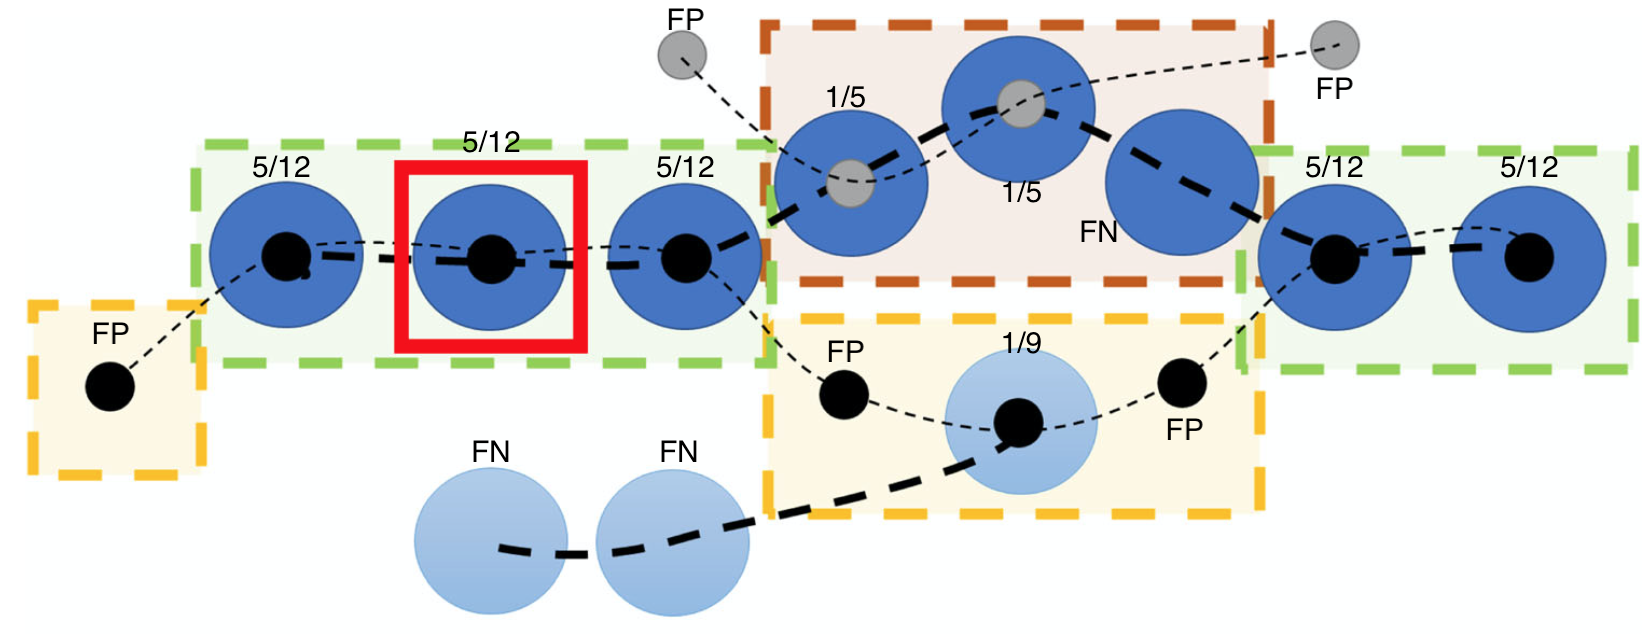
\includegraphics[width=240pt]{pics/track06.png}
	\end{figure}

	\vspace{-20pt}
	TP: 8; FP: 5; FN: 3
	\begin{itemize}
	\item ({\color{MidnightBlue}BLUE}, black): TPA=5, FPA=1+3, FNA=2+1, $\mathcal A= 5/12$
	\item ({\color{MidnightBlue}BLUE},\,\, {\color{gray}gray}): TPA=2, FPA=0+2, FNA=5+1, $\mathcal A=2/10$
	\item ({\color{cyan}CYAN}, black): TPA=1, FPA=5+3, FNA=0+2, $\mathcal A=1/11$
	\end{itemize}

	\vspace{-10pt}
	\[
		\text{HOTA} = \sqrt{\dfrac{8}{8+5+3} \cdot \dfrac{5/12*5 + 2/10*2 + 1/11*1}{8}} \approx 40.1\%.
	\]

\end{frame}

\section{The Metrics}

\begin{frame}
	\frametitle{Metrics for Evaluating Trackers}
			
	Again, we recall that \emph{performance of object trackings is based 
	on the result of detections}.
			
	\vspace{5pt}

	Hence {\bf metrics for evaluating trackers} should concern about the three aspects:
	\begin{itemize}
		\item detections;%: measure accuracies of detection
		\item associations; and%: measure accuracies of positions of correct predictions
		\item localizations.%: measure accuracies of the correct associations of objects
	\end{itemize}

	\quad

	In the following, we'll re-state the definitions of the
	metrics introduced before and see what's happened if the similarity threshold
	varies.
	

\end{frame}

% \subsection{CLEAR-MOT: MOTA and MOTP}

\begin{frame}
	\frametitle{CLEAR-MOT: MOTA and MOTP scores}
			
	% {\scriptsize\tt K. Bernardin \& R. Stiefelhagen, Evaluating Multiple Object Tracking Performance:%
	% The CLEAR MOT Metrics.}
			
	Given a similarity threshold $\alpha\in (0,1)$.
			
	\vspace{4pt}
			
	{\bf MOTA (multiple object tracking accuracy)} is calculated through
	\emph{optimizing the value}
	\[
		\text{MOTA}_\alpha :=
		\max_{\Pi_\alpha}
		\left\{1 - \dfrac{|\text{FN}_{\Pi_\alpha}| + |\text{FP}_{\Pi_\alpha}| + |\text{IDSW}_{\Pi_\alpha}|}{|\text{gtDet}|}\right\}
	\]
	among all matchings $\Pi_\alpha$ with $\mathcal S(c)\geq \alpha$ for all matched $c\in\Pi_\alpha$.
			
	\vspace{4pt}
			
	\emph{\color{blue} The FN, FP term measure the accuracy of detections.} \\
	\emph{\color{olive} The IDSW term measures the accuracy of associations.}
			
	\vspace{4pt}
		
	% Remark: under $\alpha$, the matching is taken to optimize $|\text{TP}|$ as well.
			
\end{frame}

\begin{frame}
	\frametitle{CLEAR-MOT: MOTA and MOTP scores}
			
	As the MOTA score is achieved by some matching $\Pi_\alpha$, {\bf MOTP (multiple object tracking precision)}
	is calculated as follows:
	\[
		\text{MOTP}_\alpha =
		\dfrac{\sum_{(g,p)\in\text{TP}_{\Pi_\alpha}}\mathcal S(g,p)}{|\text{TP}_{\Pi_\alpha}|}.
	\]
	\emph{\color{red} MOTP measures the accuracy of localizations of detections}.
			
	\quad
			
	% As mentioned before, if the MOTA value is low,
	% then somehow it cannot be distinguished that
	% the detections are not good or the tracking results are not good.
			
	\vspace{5pt}
		
	$\alpha\nearrow$ $\Rightarrow$ $|\text{FN}|, |\text{FP}|, \mathcal S \nearrow$,
	$|\text{TP}| \searrow$ $\Rightarrow$ MOTP $\nearrow$.

	\vspace{5pt}

	$|\text{IDSW}|, \text{MOTA}$ $?$
	
\end{frame}

\begin{frame}
	\frametitle{The ID Metrics}
			
	Under a similarity threshold $\alpha$, the id-metrics are calculated through
	\emph{optimizing the quantity $|\text{IDTP}|$ among matchings $\mathfrak P$}
	in trajectory level as follows:

	\vspace{-15pt}
	\begin{align*}
		\text{ID-Precision} := & ~ \max_{\mathfrak P} \dfrac{|\text{IDTP}|}{|\text{IDTP}| + |\text{IDFP}|}, \\
		\text{ID-Recall} :=    & ~ \max_{\mathfrak P}\dfrac{|\text{IDTP}|}{|\text{IDTP}| + |\text{IDFN}|},  \\
		\text{IDF1} :=         &                                                                            
		~ \max_{\mathfrak P}\dfrac{|\text{IDTP}|}{|\text{IDTP}| + 0.5|\text{IDFP}| + 0.5|\text{IDFN}|}.
	\end{align*}

	Note that these metrics mainly focus on the {\color{olive}\emph{tracking accuracies}}.

	\vspace{5pt}

	$\alpha\nearrow$ $\Rightarrow$ $|\text{IDTP}|\searrow$,
	$|\text{IDFP}|$, $|\text{IDFN}|$ ID-Precision, ID-Recall, ID-F1 $?$

\end{frame}

\begin{frame}
	\frametitle{The HOTA metrics}
		
	The {\bf HOTA (higher order tracking accuracy)} score for a threshold $\alpha$ is defined by
	optimizing the following value among matchings in the detection level:
	\[
		\text{HOTA}_\alpha := 
		\max_{\Pi_\alpha} \sqrt{\dfrac{\sum_{c\in\text{TP}} \mathcal A(c) }{|\text{TP}|+|\text{FN}|+|\text{FP}|}},
	\]
	where $\mathcal A(c)$ is defined by
	\[
		\mathcal A(c) = \dfrac{|\text{TPA}(c)|}{|\text{TPA}(c)|+|\text{FPA}(c)|+|\text{FNA}(c)|}.
	\]
	Note that all measures TP, FP, FN, TPA, FPA, FNA depend on matching $\Pi_\alpha$.
		
\end{frame}

\begin{frame}
	\frametitle{The HOTA metrics}
	The HOTA score is defined in a double Jaccard indices way.
	It can be divided into multiples of two values:
	Once the matching $\Pi$ is defined,
	\[
		\text{AssA}_\alpha = \dfrac{1}{|\text{TP}|} \sum_{c\in\text{TP}} \mathcal A(c), \ \ 
		\text{DetA}_\alpha = \dfrac{|\text{TP}|}{|\text{TP}| + |\text{FP}| + |\text{FN}|}.
	\]
	Then we can recall the formula:
	\[
		\text{HOTA}_\alpha = \sqrt{\text{AssA}_\alpha \cdot \text{DetA}_\alpha}.
	\]
	The two scores indicate the {\color{olive}\emph{accuracy of tracking associations}}
	and the {\color{blue}\emph{accuracy of detections}}.
\end{frame}

\begin{frame}
	\frametitle{The HOTA metrics}
		
	Similarly to MOTP, by the same matching $\Pi_\alpha$,
	the \emph{\color{red} localization score} in HOTA is defined by
	\[
		\text{LocA}_\alpha = \dfrac{\sum_{c\in\text{TP}} \mathcal S(c)}{|\text{TP}|}.
	\]
	As a remark, $\text{AssA}_\alpha$ and $\text{LocA}_\alpha$ are not well-defined
	if $\text{TP} = \emptyset$.

	\quad

	Furthermore, the numerator can be changed to another metric for evaluating localizations
	(i.e. IoU, $\max\{1-\text{dist},0\}$, \ldots).
		
\end{frame}

\begin{frame}
	\frametitle{Matching During Calculation of HOTA scores}

	Note that when applying the CLEAR-MOT or the id-metrics,
	the optimization among all matchings can be done by a greedy method.

	\vspace{5pt}

	For example, in MOTA score, the optimizing matching can be done
	frame-by-frame:
	\begin{itemize}
	\item We can optimize the number of TPs by a Hungarian algorithm.
	\item Inside a frame, if a detection can be matched to more than one
		ground-truth candidates, then we can choose one by looking up
		matchings in the previous frame and trying to minimize $|\text{IDSW}|$.
	\end{itemize}

	However, there's no greedy algorithms for calculating HOTA scores.
	
\end{frame}

\begin{frame}
	\frametitle{Matching During Calculation of HOTA scores}

	The problem is that if we want to determine the matching in a frame,
	the optimizing process in this frame should consider associations and matchings in other frames.

	\vspace{5pt}

	Hence as an alternative, we may do a {\bf pre-match}: that is, to calculate
	the framewise similarity scores and numbers of {\bf possible matches}
	during all frames of all pairs of objects.

	\vspace{5pt}

	Then the approximate tracking accuracies $\mathcal A_{\rm max}$
	of a pair $c=(g,p)$ is calculated by TPA, FPA and FNA obtained from
	the possible matches, i.e.
	\[
		\mathcal A_{\rm max}(c) = 
		\dfrac{\scriptsize\text{number of possible matches of gtId($g$) and prId($p$) during all frames}}{
			\text{\scriptsize number of frames that gtId($g$) and prId($p$) appears}.
		}
	\]

\end{frame}


% \section{Implementation of HOTA metrics}

\begin{frame}
	\frametitle{Possible Matches Counts}

	Inside a frame, similarity scores of ground-truths and detections are given.
	The {\bf possible matches counts} inside a frame
	is calculated as an IoU, and seemed as the expectation values of matches.
	\begin{align*}
	\begin{bmatrix}	
	0.8                       & 0                       & 0.1                     \\
	0.5                       & 0.3                     & 0                       
	\end{bmatrix}
	\ \stackrel{\text{IoU}}{\Rightarrow}\ 
	\begin{bmatrix}
	\frac{0.8}{0.8+0+0.1+0.5} & 0                       & \frac{0.1}{0.8+0+0.1+0} \\
	\frac{0.5}{0.8+0.5+0.3+0} & \frac{0.3}{0+0.5+0.3+0} & 0                       
	\end{bmatrix} \\
	\text{(possible matches count inside a frame)}~ \Rightarrow ~ 
	\begin{bmatrix}
	4/7                       & 0                       & 1/9                     \\
	5/16                      & 3/8                     & 0                       
	\end{bmatrix}
	\end{align*}

	Then the possible matches counts of all pairs of ground-truths and detections
	are accumulated after computing the IoU of similarities during all frames.

	Finally we can obtain $\mathcal A_{\rm max}(c)$ for
	all $c\in\text{TP}$.

\end{frame}

\begin{frame}
	\frametitle{Actual Matching by Optimization $\mathcal A_{\rm max}$}

	The actual matching is done by
	optimizing the approximate score frame-by-frame.
	\[
		\Pi^{(f)} := 
		\text{argmax}\left\{ \sum\limits_{c\in\text{TP}^{(f)}} \mathcal A_{\rm max}(c) \right\}.
	\]

	Then calculate the association scores by this `actual matching'.

	\vspace{3pt}

	From the paper author's code, for convenience, 
	the matching under threshold $\alpha$, $\Pi_\alpha$, is done by
	filter out matched pairs whose similarities are less than $\alpha$.

	\vspace{5pt}

	Finally, the (approximate) HOTA$_\alpha$ and related scores
	is obtained according to the matching.

\end{frame}

\begin{frame}
	\frametitle{The Integrated HOTA Scores}

	As mentioned before, when $\alpha\nearrow$,
	the number of TP pairs may decrease while numbers of FP and FN may increase.
	But we're not sure that
	the measures in tracking associations are likely to increase or decrease.

	\quad

	Hence the integrated HOTA scores are measured in different levels of
	similarity thresholds $\alpha$'s:
	\begin{align*}
		\text{HOTA} & = \int_0^1\text{HOTA}_\alpha\ d\alpha
		~ \approx ~ \dfrac1{19}\sum_{\alpha_i\in\{0.05,\atop \ldots,0.95\}}
		\text{HOTA}_{\alpha_i}. \\
		\text{LocA} & = \int_0^1\text{LocA}_\alpha\ d\alpha
		~ \approx ~ \dfrac1{19}\sum_{\alpha_i\in\{0.05,\atop \ldots,0.95\}}
		\text{LocA}_{\alpha_i}.
	\end{align*}
\end{frame}

\begin{frame}
	\frametitle{Drawback of HOTA metrics}
	
	\begin{itemize}
	\item HOTA metrics can not deal with realtime tracking results
		since it needs measures of global associations.
	\item The accuracies of tracking associations can not distinguish
		how long-lasting the tracker is.
	\end{itemize}

	\begin{figure}
		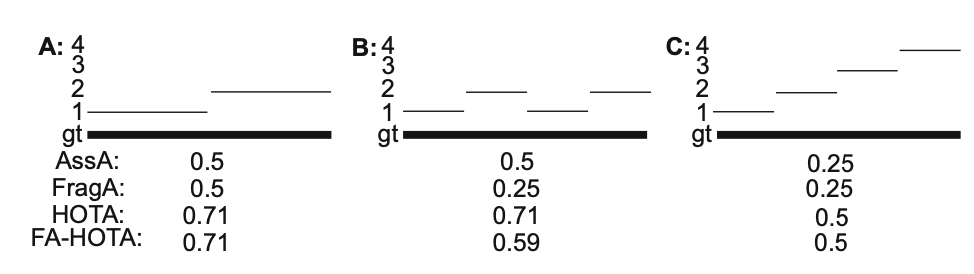
\includegraphics[width=240pt]{pics/track05.png}
		\caption{More fragmentations with the same HOTA scores.}
	\end{figure}

\end{frame}



\begin{frame}
	\frametitle{Reference}

	\scriptsize

	\begin{minipage}{190pt}
	\begin{itemize}
	\item {\sf J. Luiten, A. O\u{s}ep, P. Dendorfer, P. Torr, A. Geiger \& L. Leal-Taix\'e},
		\emph{HOTA: A Higher Order Metric for Evaluating Multi-object Tracking}, International Journal of Computer Vision (2021).
	\item {\sf R. Kasturi, et al.},
		\emph{Framework for Performance Evaluation of Face, Text, and Vehicle Detection and Tracking in Video:
		Data, Metrics, and Protocol}, IEEE Transactions on Pattern Analysis and Machine Intelligence,
		Vol. 31, No. 2, Feb. 2009.
	\end{itemize}
	\end{minipage}
	\begin{minipage}{110pt}
		\begin{figure}
			
\includegraphics[width=110pt]{pics/thank_you.png}
		\end{figure}
	\end{minipage}

\end{frame}

\end{document}